\section{\LaTeX\ versus traitements de texte}

\subsection{Traitements de texte}
\begin{frame}

Word, OpenOffice, LibreOffice, Apple Pages etc:

\begin{itemize}
  \item Stockent structure logique de votre texte dans un fichier
  \item Affichent à l'écran le rendu physique
\end{itemize}

\end{frame}

\begin{frame}
Conséquences:
\begin{itemize}
  \item Qualité typographique faible (\enquote{gris typographique}).
  \item Tendance des rédacteurs à se concentrer sur forme plutôt que fond, à ne pas tirer profit des styles.
  \item Affichage en direct des résultats :  travail ralenti.

\end{itemize}
\end{frame}

\subsection{Avantages de \LaTeX}
\begin{frame}
\LaTeX\ procède en deux étapes:

\begin{itemize}
  \item Rédaction dans un éditeur de texte. On structure le document à l'aide de commandes.
  \item Affichage à la fin grâce à un compilateur qui produit un PDF.
\end{itemize}

\end{frame}
\begin{frame}
  Permet :
  \begin{itemize}
    \item Une meilleure typographie, sans avoir besoin d'apprendre la PAO.
    \item Une séparation stricte du sens et de la forme.
  \end{itemize}
\end{frame}

\begin{frame}
  Mais aussi :
  \begin{itemize}
      \item Pérennité des formats en entrée (.tex) comme en sortie (.pdf).
      \item Automatisation de certaines tâches.
      \item Interaction avec d'autres logiciels, par ex R pour les statistiques.
      \item Travail collaboratif à l'aide de logiciels spécialisés (par ex. GIT).
  \end{itemize}
\end{frame}

\subsection{\XeLaTeX, une forme particulière de \LaTeX}
\begin{frame}
  \begin{itemize}
    \item Gestion native de l'Unicode et des polices OpenType
    \item Particulièrement adapté aux personnes qui travaillent sur des langues non latines.
  \end{itemize}
\end{frame}

\subsection{Avantage dans le domaine des SHS}

\begin{frame}
  \begin{itemize}
    \item Gestion bibliographique, avec ou sans relation avec Zotero. 
    \item Gestion des éditions critiques.
    \item Construction de schéma (arbre généalogique par ex.)
    \item Interaction directe avec R.
  \end{itemize}
\end{frame}

\subsection{Éditeurs de texte versus traitement de texte}

\begin{frame}
  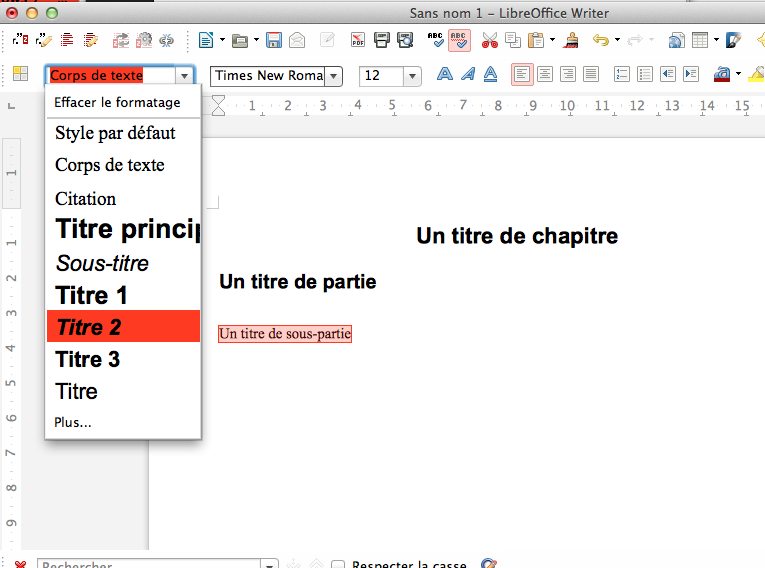
\includegraphics[width=\textwidth]{wysiwyg.png}
\end{frame} 
\begin{frame}
  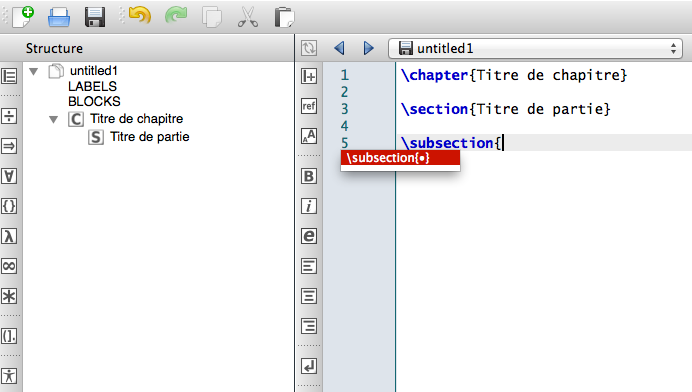
\includegraphics[width=\textwidth]{editeur.png}
\end{frame}

\subsection{L'apprentissage ?}

\begin{frame}
	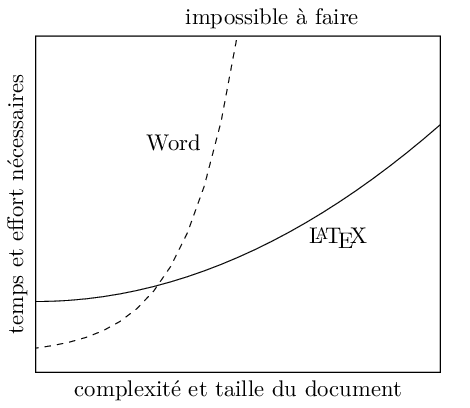
\includegraphics[width=\textwidth]{latex1_chart_fr.png}
	\url{http://www.plpeeters.com/blog/article/introduction-a-latex-110.html}
\end{frame}

\subsection{Exemple de rendu typographique}
\begin{frame}
  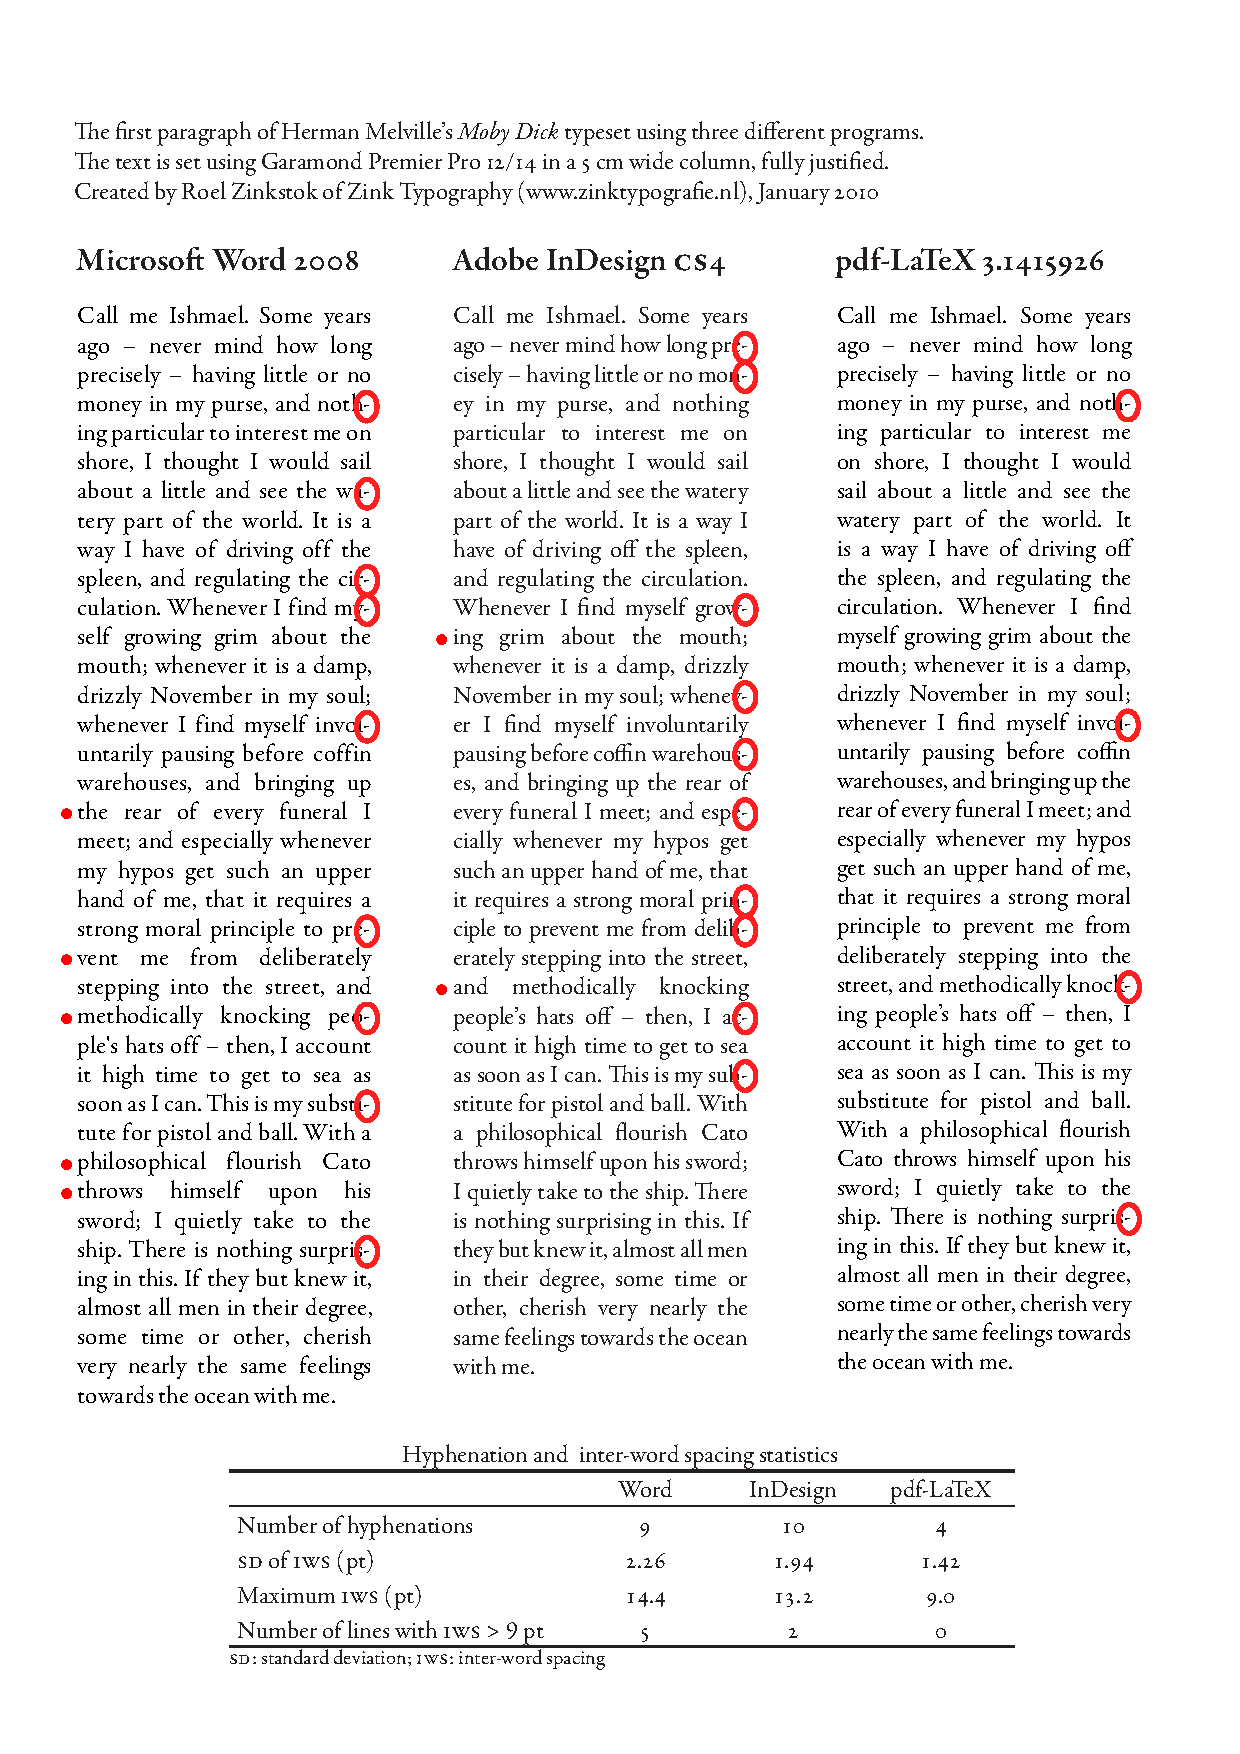
\includegraphics[width=\textwidth]{comparison.pdf}
  \url{http://www.zinktypografie.nl/comparison.pdf}
\end{frame}
